\chapter{Evaluation}
\label{chapter:evaluation}

Performance evaluation \\
- Methodology \\
- How/what is tested \\
    - Hypervisors
- Results \\
- Evaluation \\
- Comparison to other providers (AWS, GCP...) \\






The extra layer of security provided by Kata Container's micro-VM comes with a price of degraded performance and computational overhead. Previous work, such as \cite{Kumar2020} and \cite{EverartsdeVelp2020} have examined the performance, when compared Kata Containers against native runtime runC, the most common OCI-compliant runtime. In these two papers, Kata Containers architecture design results in performance decrease in IO throughput, and in memory and CPU utilization. However, the results in these papers are highly dependant on the specific test environment and do not take in account the latest development of Kata Containers performance provided by the runtime version 2.0 released in December 2020. In this paper, the system performance evaluated in environment simulating a telco architecture, which is discussed in Section \ref{section:test_architecture}.

\section{Test architecture}
\label{section:test_architecture}

The test environment simulates multiple relations that are most common in a telco environment. The test environment cluster is described in Figure \ref{fig:TestArchitectureCluster} and Node 1 in more detail in Figure \ref{fig:TestArchitectureNode}. The cluster consists of two nodes, which both have two containers inside. The difference between nodes are pods, with Node 1 consisting of a single pod with two containers inside, and Node 2 consist of two pods with a single container deployed to each pod. The purpose of the heterogeneous environment is to evaluate performance of a single container or between two containers in various scenarios.

\begin{figure}[ht]
  \begin{center}
    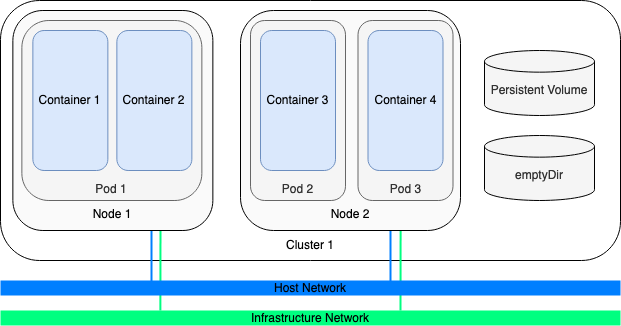
\includegraphics[width=13.5cm]{LaTeX/images/TestArchitectureCluster.png}
    \caption{Kubernetes test cluster overview}
    \label{fig:TestArchitectureCluster}
  \end{center}
\end{figure}

\begin{figure}[ht]
  \begin{center}
    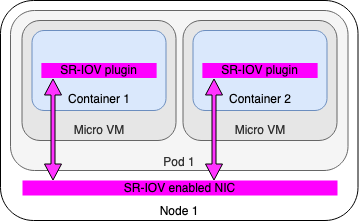
\includegraphics[width=13.5cm]{LaTeX/images/TestArchitectureNode.png}
    \caption{Node test cluster with two containers in a single pod}
    \label{fig:TestArchitectureNode}
  \end{center}
\end{figure}

Container - container inside pod

Container - container between pods

Container - container across nodes and a pods

Container - storage


The cluster consists also two storage options, which are Persistent Volume (PV) and emptyDir. PV 
    - What is emptyDir?
    - PV (block). Why block? Link to K8s docs.
    - Volumes mounted.
    - Multi-tenancy? Write many?

Networking
    - Two networks. What is the difference?
    - Access to storage not via network, unless NFS(?).






\section{Methodology}

The test environment is hosted by a dedicated server which is built and tailored to support edge and far-edge cloud deployments.


\section{Results}

\section{Evaluation}

\section{Benchmark from other platforms}